\documentclass{jarticle}
\usepackage{amsmath}
\usepackage{psfrag}
\pagestyle{empty}
\def\vect#1{\boldsymbol{#1}}

\begin{document}
%%dvips(k) -Ppdf -E ���ä��� EPS �ˤ��Ƥ��顤�����ᥤ��� LaTeX �ե����������
\psfragscanon
\psfrag{O}[][]{$O$}
\psfrag{U}[][]{$U$}
\psfrag{V}[][]{$V$}
\psfrag{Ud}[][]{$U'$}
\psfrag{Vd}[][]{$V'$}
\psfrag{W}[][]{$W$}
\psfrag{vU}[][]{$\vect{u}$}
\psfrag{vV}[][]{$\vect{v}$}
\psfrag{vW}[][]{$\vect{w}$}
\psfrag{l}[][]{$l$}
\psfrag{m}[][]{$m$}
\resizebox{5cm}{!}{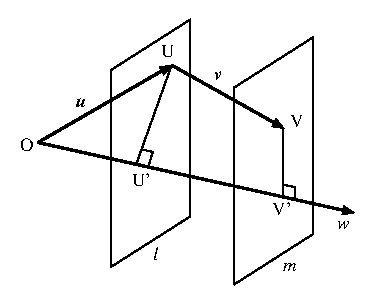
\includegraphics{scalar-product.eps}}

\end{document}
